\section{Problema 3}

\subsection{Pseudocódigo}

\begin{codebox}
\Procname{$\proc{MCD_Greedy}$ (\textbf{in} $Grafo$)}{conjuntoDomGoloso}{Conj de Vertices}
\li	vertices = lista de vertices del grafo
\li	dominantes = conjunto vacio de vertices
\li	\textbf{Mientras} no esten todos los vertices cubiertos \Do
\li 		Ordeno los vertices por la cantidad adyacentes que tenga no cubiertas (sin dominar), de mayor a menor.
\li 		Elijo como dominante al primero de la lista y lo agrego al conjunto de \textbf{dominantes}
\li 		Saco de la lista de vertices al elegido
\li 		Actualizo los nodos del grafo, disminuyendo la cantidad de \texit{grado sin dominar} de los adyacentes al elegido, y de los adyacentes a estos.
	\End
\li	return \textbf{dominantes}
\end{codebox}

\subsection{Orden de complejidad}

La complejidad de mi algoritmo es de 2^n * n³. Voy a demostrarlo por inducción:

Caso Base:

n = 1, si n tiene un solo nodo ver si es dominante me cuesta O(1) ya que recorrer los vertices del grafo original es una sola iteracion y no es posible recorrer sus aristas. Luego divido en el caso en el que uso a ese nodo en el conjunto dominante y el caso en que no. El caso en que no al no tener mas nodos con cual probar me va a devolver el grafo original y el otro caso también ya que el grafo original era el que contenía únicamente a ese nodo. Ambos casos ver si el conjunto es dominante cuesta O(1) ya que tiene a lo sumo una iteración para hacer. Por lo tanto el algoritmo costaría O(1) que es igual a O(2¹*1³).

Hipótesis inductiva:

Supongo que con n nodos la complejidad es 2^n * n³

Paso inductivo:

Quiero ver que con n+1 nodos la complejidad pertenece a 2^(n+1)*(n+1)³

Ver si el conjunto vacío es dominante me cuesta O(1) ya que en la primera iteración del grafoOriginal no es posible encontrar ningún vertice en el conjunto dominante o adyacente a él. Luego obtengo un nodo del grafo (grafo en el que me guarde todos los vertices, no el origianl) y busco el minimo conjunto dominante agregando ese nodo al conjunto o no, esto por hipótesis inductiva me cuesta 2 * (2^n * n³), ya que tengo que calcular 2 veces el conjunto minimo para n nodos. Por lo tanto la complejidad me termina costando  2^(n+1)*n³ y esto pertence a 2^(n+1)*(n+1)³. Con lo cual queda demostrada la complejidad.

Notar que esta complejidad esta por encima de la complejidad exacta, ya que el n³ variaría en cada iteración dependiendo de la cantidad de nodos en el conjuntoDominante.


\subsection{Peor Caso}

Como el algoritmo es exacto y recorre todas las soluciones posibles siempre obtiene la mejor de ellas. Por lo tanto no existe una 'peor' instancia
en la que la solución devuelta sea sub-óptima, siempre devuelve la mejor.

\subsection{Tests y análisis}

En los siguientes gráfico podemos observar que la cantidad de ciclos y el tiempo crecen notablemente a medida que el grafo tiene cada vez mas nodos.\\
Esto es debido a que, como dijimos anteriormente, la complejidad es polinomica en el tamaño de la entrada (en este caso, la cantidad de nodos 
del grafo) y no existe un mejor o peor en caso en el cual la complejidad sea mucho menor a O(n^4). Por esto es que tanto en el grafico de tiempos
 como en el de ciclos se puede observar claramente que la complejidad es exponencial.

\begin {center}
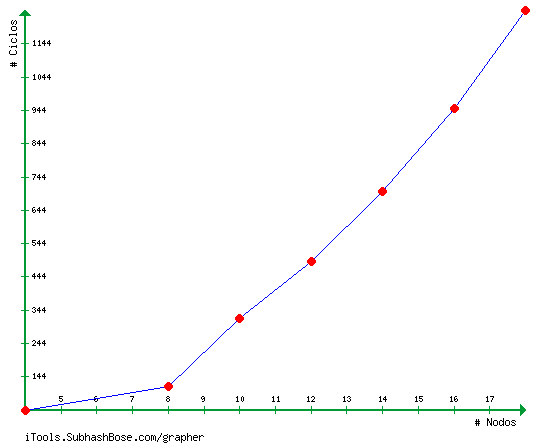
\includegraphics[width=8cm]{./graficos/goloso_1.png}
% grafico.eps: 0x0 pixel, 300dpi, 0.00x0.00 cm, bb=50 50 410 302
\end {center} 

\begin {center}
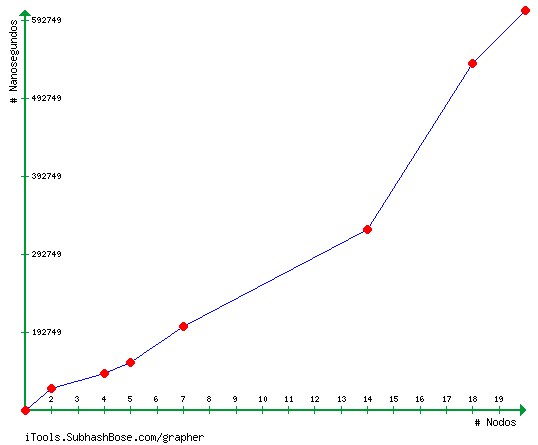
\includegraphics[width=8cm]{./graficos/goloso_2.png}
% grafico.eps: 0x0 pixel, 300dpi, 0.00x0.00 cm, bb=50 50 410 302
\end {center}